\begin{section}{N-body Simulation of Dark Matter Density Fields}
  \label{sec:simulation}
    We use the \textsc{CUBEP$^3$M} \cite{bib:Harnois2013} to 
run 136 simulations with a box size of 300 $h^{-1}$Mpc, 
afine resolution of $1024^3$ cells and $512^3$ totally particles. The initial conditions are 
computed using the transfer function given by CAMB \cite{bib:Lewis2000} 
and then propogating the power linearly back to $z=100$ with a growth factor. The Zel'dovich approximation 
is used to calculate the displacement and velocity fields, which are 
assigned to the particles. The cosmological parameters used are $\Omega_M=0.32$, 
$\Omega_{\Lambda}=0.679$, $h=0.67$, $\sigma_8=0.83$, and $n_s=0.96$. Different seeds are used to produce 
the initial conditions for different simulations so that they are 
independent to each other.
\begin{figure*}[t!]
\centering
 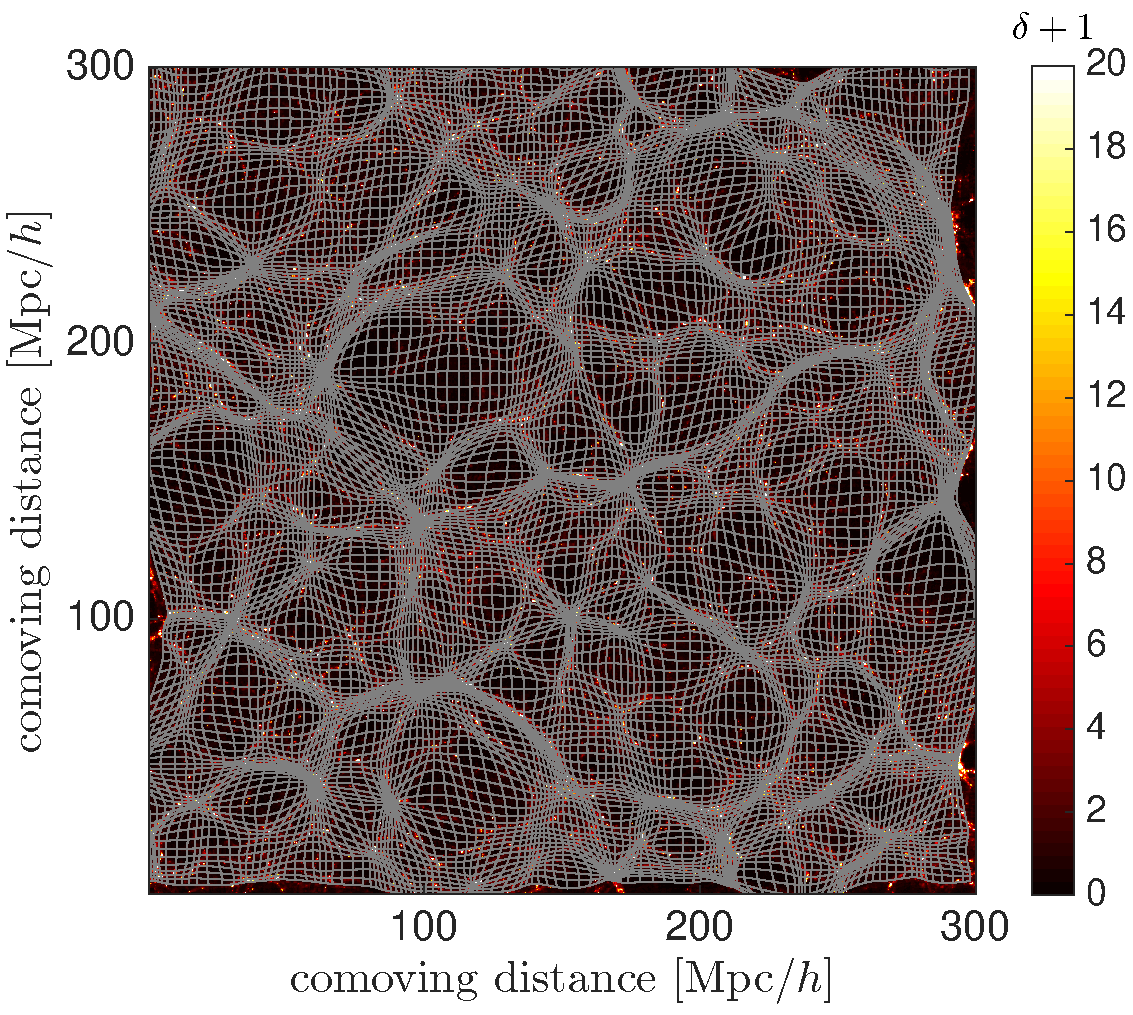
\includegraphics[width=0.9\textwidth]{sar_bbest_analysis-crop.pdf}
% \label{fig:simandrec}
   \caption{
The 2-D projection of the 
deformed grid of a sample $N$-body simulations is shown as curved white lines. The $\delta+1$ field 
on the deformed grid is shown underneath.}
 \label{fig:simandrec}
\end{figure*}

\end{section}

